\subsection{Inferenza su espressioni}
\label{sec:5-9-expression-inference}

La classe \texttt{InferenceEngine} contiene solamente proprietà e metodi statici, e non adotta lo stesso
procedimento di esplorazione dell'albero sintattico delle classi figlie di \texttt{ASTVisitor}
(visualizzazione e traduzione in \texttt{Java}): il cammino attraverso l'\textbf{AST} inizia con un metodo
di avvio per chiamate ricorsive sulle funzioni di inferenza di ciascun nodo,
a partire dal \texttt{let} delle dichiarazioni globali di un modulo.


Come già accennato nella sezione~\ref{sec:3-4-hm-type-inference}, i metodi sono molto simili all'\textit{algoritmo $\mathcal{W}$} mostrato,
e le classi ausiliarie appena descritte facilitano lo sviluppo delle funzioni di inferenza seguendo tale modello da vicino.

\noindent Ciò nonostante, si vuol descrivere brevemente l'implementazione del metodo \texttt{infer} della classe \texttt{Let},
in quanto di particolare interesse per le modifiche apportate al fine di gestire opportunamente
la ricorsione e la generalizzazione dei tipi delle funzioni.

\noindent L'inferenza per \texttt{let}, presentata nel Codice~\ref{lst:5-9-let-inference-java}, si divide in 4 fasi:
\begin{itemize}
    \item linee 3-21, inizializzazione del contesto:
          \begin{itemize}
              \item creazione di una mappa per le posizioni delle dichiarazioni;
              \item copia del contesto originale;
              \item controllo di dichiarazioni duplicate;
              \item aggiornamento del contesto con schemi di tipo temporanei;
          \end{itemize}
    \item linee 23-43, inferenza sulle dichiarazioni locali:
          \begin{itemize}
              \item initializzazione della sostituzione;
              \item inferenza per ogni dichiarazione;
              \item unificazione tra tipi noti (compresi quelli temporanei) e tipi inferiti, progressiva composizione delle sostituzioni;
              \item applicazione della sostituzione al contesto;
          \end{itemize}
    \item linee 45-53, generalizzazione dei tipi:
          \begin{itemize}
              \item propagazione delle sostituzioni e chiamata alla funzione \texttt{generalize};
              \item controllo del tipo definito dallo sviluppatore;
              \item aggiornamento del contesto;
          \end{itemize}
    \item linee 55-60, inferenza sull'espressione principale:
          \begin{itemize}
              \item chiamata ricorsiva;
              \item composizione finale delle sostituzioni;
              \item propagazione delle sostituzioni e assegnamento del tipo per il nodo \texttt{let}.
          \end{itemize}
\end{itemize}

\newpage

\begin{lstlisting}[caption={Metodo di inferenza per espressioni \texttt{let}}, style=javaCode, label={lst:5-9-let-inference-java}]
@Override
public Utils.Tuple@<Substitution, Type@> infer(Context ctx) {
    // check for duplicate declarations within the same let
    Map@<String, InputPosition@> declarationPositions = new HashMap@<@>();

    Context newCtx = new Context(ctx);

    for (Declaration decl : localDeclarations.declarationList) {
        if (declarationPositions.containsKey(decl.id))
            InferenceEngine.reportError(decl.inputPosition,
                String.format("variable '%s' already declared at %s",
                    decl.id, declarationPositions.get(decl.id)));
        else {
            declarationPositions.put(decl.id, decl.inputPosition);

            // while also updating the context with placeholder schemes,
            // so that self and mutual recursion can be handled
            newCtx.bind(decl.id,
                new Scheme(Collections.emptySet(), InferenceEngine.newTypeVariable()));
        }
    }

    // proceed to infer all local declarations
    Substitution subst = Substitution.EMPTY;

    for (Declaration decl : localDeclarations.declarationList) {
        Utils.Tuple@<Substitution, Type@> declInference = decl.expression.infer(newCtx);
        try {
            // unifying types of known bindings,
            // gradually composing substitutions and updating context
            subst = subst.compose(declInference.fst())
                .compose(newCtx.bindingOf(decl.id).type
                    .applySubstitution(subst)
                    .unify(declInference.snd())); // could throw TypeException

            decl.expression.type = declInference.snd().applySubstitution(subst);

            newCtx = newCtx.applySubstitution(subst);
        } catch (TypeException e) {
            InferenceEngine.reportError(decl.inputPosition, e.getMessage());
            decl.expression.type = Type.Error.INSTANCE;
        }
    }

    // finally generalize all types and check against actual user-defined schemes
    for (Declaration decl : localDeclarations.declarationList) {
        decl.expression.propagateSubstitution(subst);

        Scheme expectedScheme = decl.expression.type.generalize(newCtx);
        decl.checkScheme(expectedScheme);

        newCtx.bind(decl.id, decl.scheme());
    }

    // now it's possible to infer the expression type
    Utils.Tuple@<Substitution, Type@> exprInference = expression.infer(newCtx);

    subst = subst.compose(exprInference.fst());
    type = exprInference.snd().applySubstitution(subst);
    expression.propagateSubstitution(subst);

    return new Utils.Tuple@<@>(subst, type);
}
\end{lstlisting}

\newpage

\begin{lstlisting}[caption={Esempio di inferenza}, style=funxCode, label={lst:5-9-types-funx}]
main = countdown 1825

countdown : Int @-> Int
countdown = until (equalsEquals 0) (flip subtract 1) 

until p f = until1
    with
        until1 x = if p x then x else until1 (f x) fi
    out    
\end{lstlisting}

\begin{figure}
    \vspace{4mm}
    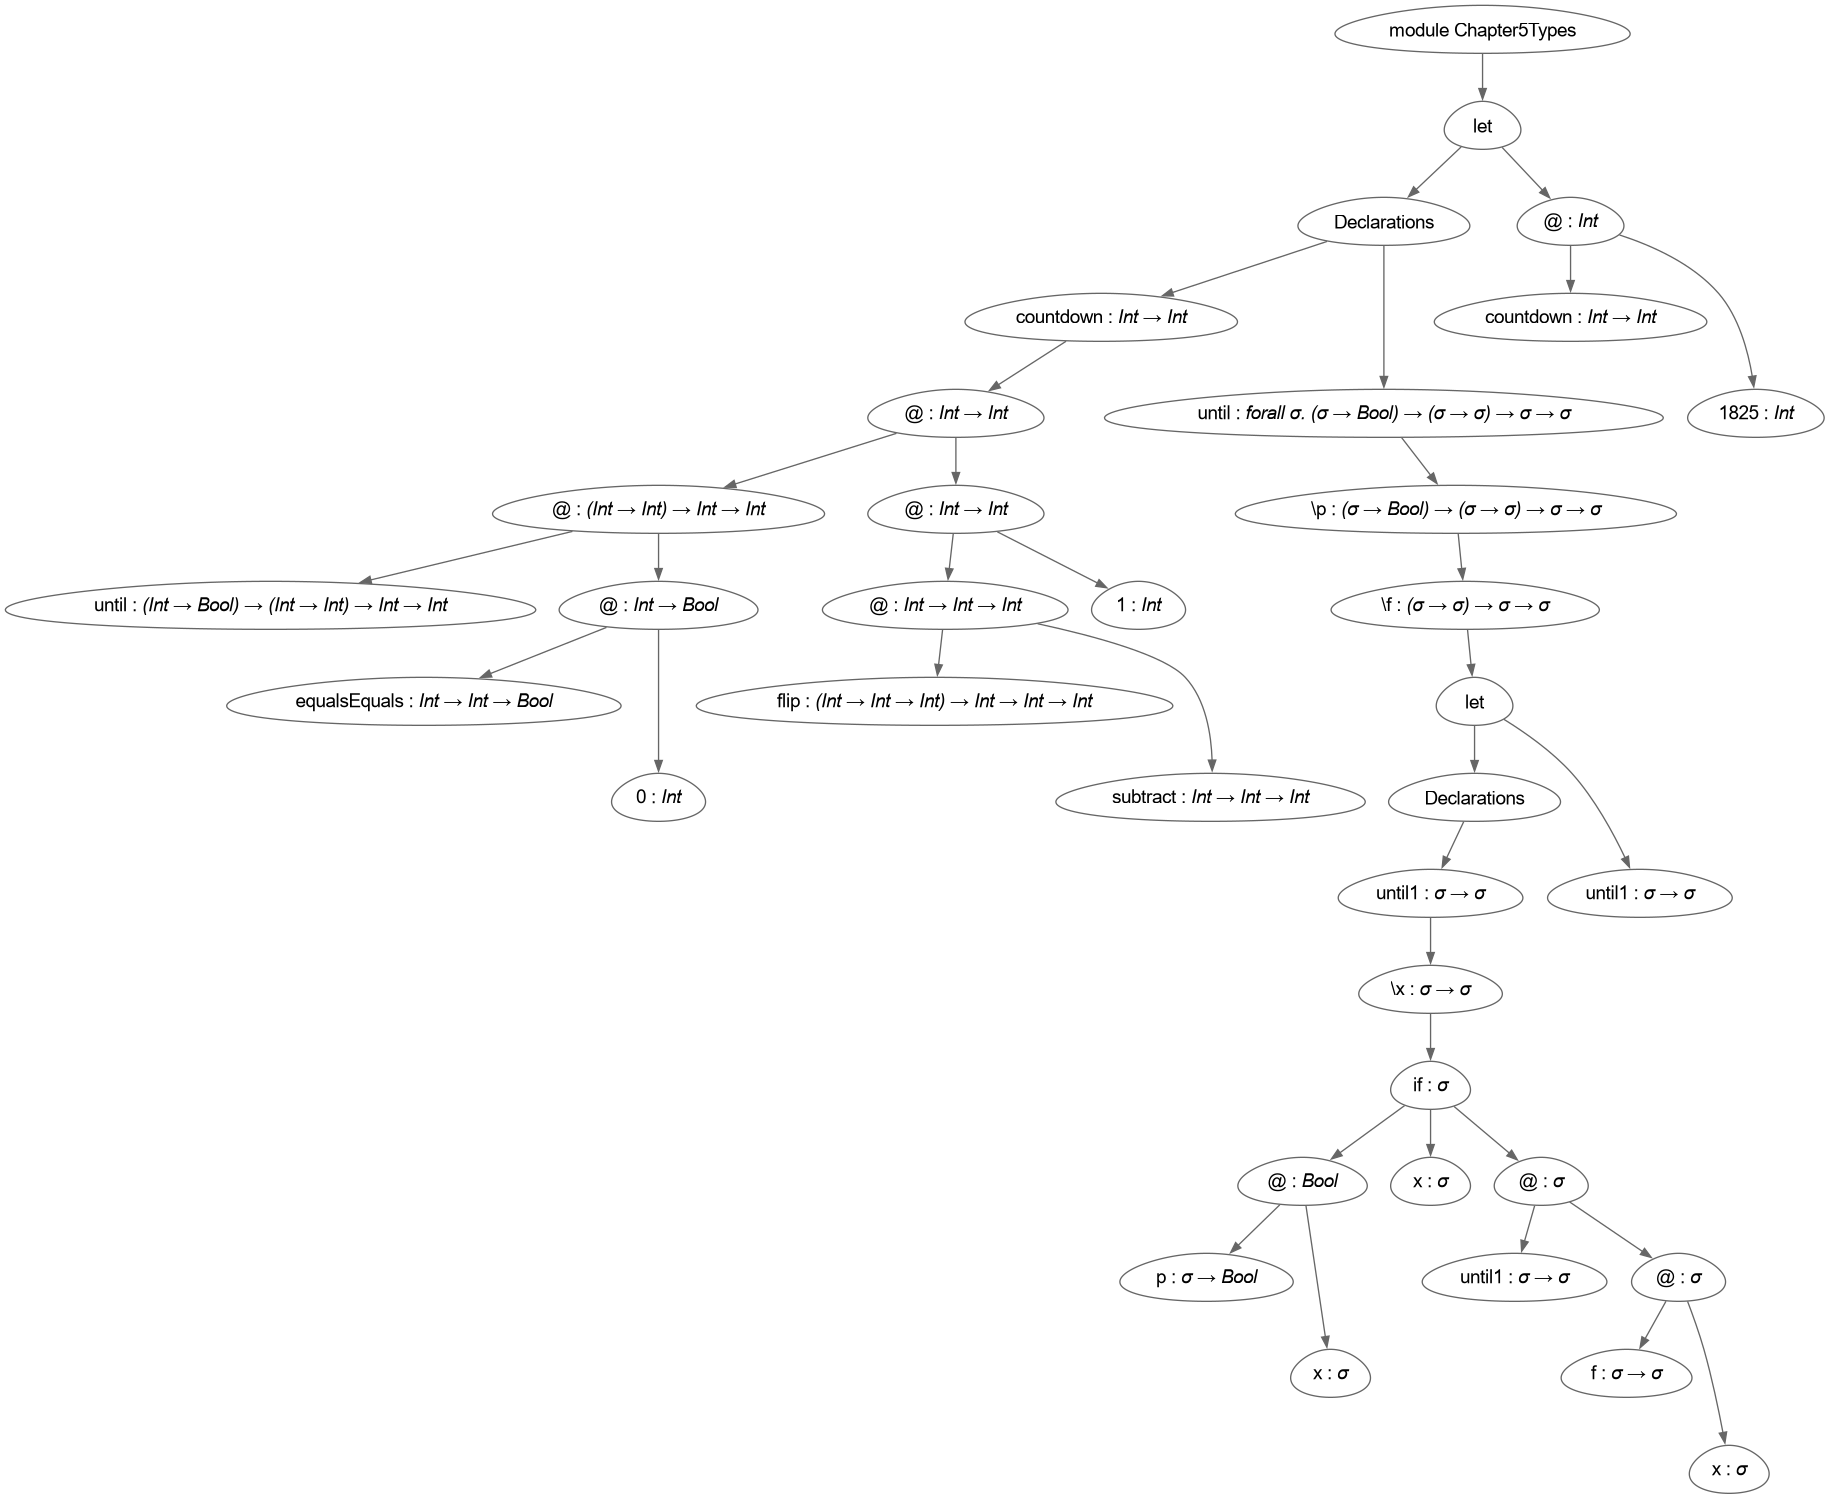
\includegraphics[width=\textwidth]{5-9-type-annotations.png}
    \caption{\textbf{AST} con annotazioni di tipo}
    \label{fig:5-9-type-annotations}
\end{figure}
